\documentclass[eikonal.tex]{subfiles}

\begin{document}

\section{Background}\label{sec:background}

\begin{figure}[t]
  \centering
  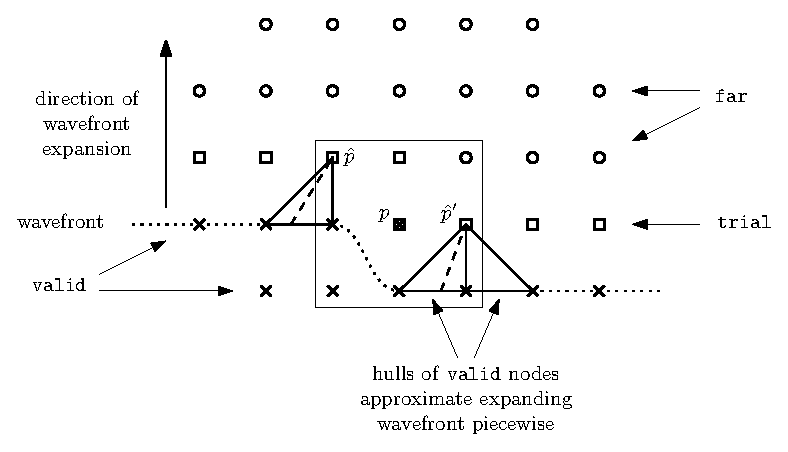
\includegraphics{overview.eps}
  \caption{The ``expanding wavefront'' is \emph{not} constructed by
    the algorithm.}
  \label{fig:overview}
\end{figure}

\subsection{Algorithms for solving the eikonal equation}

To numerically solve \cref{eq:eikonal}, first let
$\calG = \{p_i\} \subseteq \Omega$ be the set or grid of \emph{nodes}
where we would like to approximate the true solution $u$ with a
numerical solution $U : \calG \to
\overline{\mathbb{R}}_+$. Additionally, for each node $p \in \calG$,
define a set of neighbors,
$\neib(p) \subseteq \calG \backslash \set{p}$. Typically, $\calG$ is
taken to be a subset of a lattice in $\R^n$ and $\neib(p)$ to be each
node's $2n$ cardinal neighbors. With $\calG$ defined, we also define
the set of \emph{boundary nodes}, $\boundary \subseteq \calG$. It may
happen that the set $\boundary$ and $D$ do not coincide (e.g., $D$
could be a curve which does not intersect $\calG$); to reconcile this
difference, the initial value of $U(p)$ for each $p \in \boundary$
must take $g$ into account in the best way possible. This problem has
been approached in different ways, and is not the focus of the present
work (\hl{cite}). Throughout, we will assume
$\boundary = D \subseteq \calG$.

Broadly speaking, there are two competing families of solvers for the
eikonal equation: Dijkstra-like methods and fast sweeping methods. 

\subsection{Dijkstra-like algorithms}\label{ssec:dijkstra-like}
We will give a brief description of a prototypical Dijkstra-like
algorithm for solving the eikonal equation. The idea is to order the
solution of the eikonal equation dynamically so that new values are
continually computed using only fixed upwind values. This is done
using a variant of Dijkstra's algorithm for finding shortest paths in
a network, hence the name; in principal, other algorithms can be used
that have different complexity guarantees but which may offer other
performance advantages---see~\cite{chacon2012fast} for a
review. Dijkstra's algorithm is a type of \emph{label-setting method}
for finding shortest paths in a network; there are also
\emph{label-correcting methods}.

Using Dijkstra's algorithm to solve a ``continuous shortest path''
problem has been discovered in several contexts. The earliest such
development appears to be due to Mitchell, Mount, and Papadimitriou,
who used this idea to approximate geodesics on triangulated
surfaces~\cite{mitchell1987discrete} (\hl{\textbf{TODO}}: \emph{double
  check}). This was followed by Tsitsiklis who developed a first-order
semi-Lagrangian method for solving isotropic control problems on a
uniform grid~\cite{tsitsiklis1995efficient}. Finally, the fast
marching method, which uses a firs-order upwind finite difference
scheme was developed by Sethian for isotropic front
propagation~\cite{sethian1996fast}. Many variations of these methods
have since been developed. Our own development most closely resembles
Tsitsisklis's.

There are several pieces of information that need to be kept track of
in order to implement the algorithm. For each node $p$, apart from the
current value of $U(p)$, the most salient piece of information is the
\emph{state} of each node $p$, written $p$\texttt{.state}
$\in \set{\texttt{valid}, \texttt{trial}, \texttt{far}}$. The meaning
of each of these states will become clear from the following
high-level description of the algorithm:

\begin{algorithm}
  \caption{A schematic Dijkstra-like algorithm for solving the eikonal
    equation.}\label{alg:dijkstra-like}
  \begin{enumerate}[nolistsep]
  \item For each $p \in \calG$, initially set $p$\texttt{.state} $=$
    \texttt{far} and $U(p) = \infty$.
  \item For each $p \in \boundary$, set $p$\texttt{.state} $=$
    \texttt{valid}, initialize $U(p)$, and execute
    \cref{enum:set-trial,enum:update-U}.
  \item At this point, each $p \in \boundary$ is sorted by $U(p)$ in
    increasing order into a generic list or data structure called
    \texttt{front}.
  \item While there are \texttt{trial} or \texttt{far} nodes left in
    $\calG$:
    \begin{enumerate}[nolistsep]
    \item Let $p$ be the \texttt{trial} node in \texttt{front} with
      the smallest value $U(p)$.
    \item Set $p$\texttt{.state} $\gets$ \texttt{valid} and remove $p$
      from \texttt{front}.
    \item For each $\hat{p} \in \neib(p)$, set
      $\hat{p}$\texttt{.state} $\gets$ \texttt{trial} if
      $\hat{p}$\texttt{.state} $=$ \texttt{far}.\label{enum:set-trial}
    \item For each $\hat{p} \in \neib(p)$ such that
      $\hat{p}$\texttt{.state} $=$ \texttt{trial}, update
      $\hat{U} = U(\hat{p})$ and merge $\hat{p}$ into
      \texttt{front}.\label{enum:update-U}
    \end{enumerate}
  \end{enumerate}
\end{algorithm}

Computing $\hat{U}$ in \cref{enum:update-U} is left intentionally
vague. Specifying this step involves indicating how nodes in
$\neib(\hat{p})$ are to be used to compute $\hat{U}$. In the fast
marching method, an upwind finite difference stencil is used in the
sense that only nodes that are \texttt{valid} propagate information;
variations where \texttt{trial} nodes contribute have also been
considered but do not appear to improve the error in all
cases. Semi-Lagrangian methods like Tsitsiklis's group nodes in
\texttt{valid} into sets whose convex hulls partition an approximation
to the surface of the expanding wavefront and then solve local
raytracing problems involving each such group. The method presented
here operates in the same way, so this local ray-tracing idea is
depicted in \cref{fig:overview}.

The exact sequencing and details of some of the steps of
\cref{alg:dijkstra-like} is variable. Our intent here is to give a
birds-eye view of the algorithm---for concrete details, a suitable
reference should be consulted~\cref{sethian1999level}. In addition to
\cref{enum:update-U}, algorithm \cref{alg:dijkstra-like} is generic in
the following ways:
\begin{itemize}
\item As we mentioned before, there are different ways of computing
  $\boundary$ and subsequently approximating the initial value of $U$
  for $p \in \boundary$ using $g$ (\hl{cite}), the initial value for
  $\left. s \right|_D$.
\item How we keep track of the node with the smallest value is
  variable: most frequently, as in Dijkstra's algorithm, a heap
  storing pointers to the nodes is used, leading to $O(N \log N)$
  update operations overall, where $N$ is the number of nodes.
\item Related to the foregoing point, the arrangement of the nodes
  (into a grid or otherwise) varies; hence, the neighborhood of each
  node varies. This naturally affects the update
  procedure. Dijkstra-like methods have been extended to manifolds and
  unstructured meshes~\cite{sethian2000fast}.
\end{itemize}
Still other problems can be solved using Dijkstra-like algorithms: the
Hamilton-Jacobi equation, an isotropic generalization of the eikonal
equation, can be solved using the ordered upwind
method~\cite{sethian2003ordered}, and the quasipotential of a
nongradient stochastic differential equation can be computed using the
ordered line integral method~\cite{dahiya2017ordered}. This latter
approach is the progenitor of the current work.

\subsection{Fast sweeping methods} Another approach to solving a
discretized version of \cref{eq:eikonal} is the fast sweeping
method~\cite{tsai2003fast,zhao2005fast}. Unlike Dijkstra-like methods,
which are direct solvers, the fast sweeping method is an iterative
solver using an upwind scheme and varying sweep directions. For
problems where the characteristics of the solution change direction
infrequently, the algorithm obtains $O(N)$ complexity. A drawback of
the method is that the asymptotic constant for this complexity
guarantee cannot be bound a priori and depends heavily on the geometry
of the problem. Fast sweeping methods have been extended to
Hamilton-Jacobi equations~\cite{kao2004lax,tsai2003fast}, and hybrid
methods combining the fast sweeping method with a Dijkstra-like method
have been introduced~\cite{chacon2012fast,chacon2015parallel}.

\end{document}

%%% Local Variables:
%%% mode: latex
%%% TeX-master: "sisc-eikonal.tex"
%%% End:
